\documentclass{article}
\usepackage{graphicx}
\usepackage[margin=1.5cm]{geometry}
\usepackage{amsmath}

\begin{document}

\title{Wednesday Reading Assessment: Unit 0, and vectors}
\author{Prof. Jordan C. Hanson}

\maketitle

\section{Chapter 2.3 - Algebra of Vectors}

\begin{enumerate}
\item Which of the following is a correct expression for the multiplication of a scalar $a$ and a vector $\vec{p} = p_x \hat{i} + p_y \hat{j}$?
\begin{itemize}
\item A: $a\vec{p} = a p_x \hat{i} + p_y \hat{j}$
\item B: $a\vec{p} = p_x \hat{i} + a p_y \hat{j}$
\item C: $a\vec{p} = a p_x \hat{i} + a p_y \hat{j}$
\item D: $a\vec{p} = a p_x + a p_y$
\end{itemize}
\item Suppose a displacement vector $\vec{x}$ has a magnitude $|\vec{x}|$.  Which of the following best describes the quantity $\vec{x}/|\vec{x}|$?
\begin{itemize}
\item A: $\vec{x}/|\vec{x}|$ is a scalar number with the magnitude of $\vec{x}$.
\item B: $\vec{x}/|\vec{x}|$ is a vector with the magnitude of $\vec{x}$.
\item C: $\vec{x}/|\vec{x}|$ is a vector with magnitude of zero.
\item D: $\vec{x}/|\vec{x}|$ is a vector with magnitude of one.
\end{itemize}
\item Figure \ref{fig:puppies} contains a 2D coordinate system containing four vectors representing the forces with which four puppies pull a toy.  \textbf{Suppose the angles $\alpha$, $\beta$, and $\gamma$ are all 45 degrees instead of those given,} and suppose each puppy pulls with equal force.  (a) If Dug pulls with equal force as well, what angle must Dug's force vector make with the x-axis if the net force is zero?  (b) If Dug lets go and the only puppies pulling are A, B, and C, in which direction will the toy accelerate?
\begin{figure}[hb]
\center
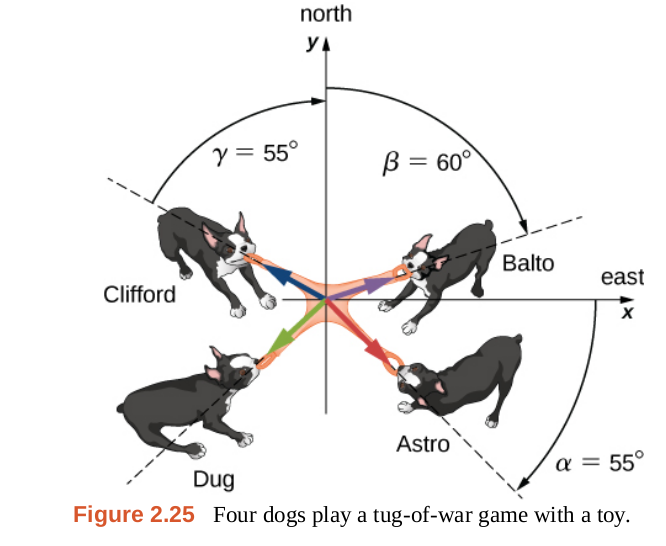
\includegraphics[width=0.5\textwidth]{figures/puppies.png}
\caption{\label{fig:puppies} A diagram of the vectors of ``force'' from four puppies pulling in different directions.}
\end{figure}
\end{enumerate}

\end{document}
